\documentclass[12pt,letterpaper]{article}
\usepackage[utf8]{inputenc}

\usepackage[spanish]{babel}
\usepackage{amsmath}
\usepackage{color}
\usepackage{algorithm}
\usepackage[noend]{algpseudocode}
\renewcommand{\algorithmicrequire}{\textbf{Entrada:}}
\renewcommand{\algorithmicensure}{\textbf{Salida:}}
\usepackage{subcaption}
\usepackage{amsfonts}
\usepackage{hyperref}
 \hypersetup{
     colorlinks=true,
     linkcolor=blue,
     filecolor=blue,
     citecolor = blue,      
     urlcolor=cyan,
     }
\usepackage{amssymb}
\usepackage{listings}

\usepackage{amsthm}
\newtheorem{theorem}{Teorema}

\usepackage{graphicx}
\usepackage[left=2cm,right=2cm,top=2cm,bottom=3.5cm]{geometry}
\setlength{\parskip}{3mm}
\title{\textsc{Práctica 6: \\ Sistema multiagente}}
\author{\textsc{Fabiola Vázquez}}

\setlength{\parindent}{0cm}
\renewcommand{\lstlistingname}{Código}
\floatname{algorithm}{Algoritmo}
\spanishdecimal{.}
\begin{document}
\maketitle

\hrule
\section{Introducción}
El objetivo de esta práctica \cite{elisapractica6} es implementar un sistema multiagente en una aplicación en epidemiología. El experimento se realiza con el software R versión 4.0.2 \cite{R} en un cuaderno de Jupyter \cite{jupyter}. 

\section{Experimento}
Se considera un cuadrado de tamaño \texttt{l}$\times$\texttt{l} en donde se posicionan \texttt{n} agentes uniformemente al azar y con una probabilidad de \texttt{pi} el agente puede estar infectado desde el inicio. En este caso se considera \texttt{l} = 1.5 y \texttt{n}=50. Además, los agentes pueden estar infectados desde el inicio con una probabilidad de \texttt{pi}. En cada iteración, denotada por \texttt{itmax}, cada uno de los agentes cambian su posición en una dirección fija y están en contacto con los demás,  por lo cual se considera una probabilidad de contagio denotada por \texttt{pc}, la cual es proporcional a la distancia euclideana entre dos agentes.

Se vacuna con probabilidad \texttt{pv} a los agentes al momento de crearlos, de esa manera no podrán ser infectados en ninguna de las iteraciones posteriores. Se varía dicha probabilidad \texttt{pv} de cero a uno en saltos de 0.05. Se consideran 100 iteraciones y 100 réplicas de cada variación. 

El cuadro \ref{datos} se muestra un fragmento de los datos que se obtuvieron en el experimento. La figura \ref{box1} muestra los gráficos de caja variando la probabilidad \texttt{pv}. Como se puede apreciar en dicha figura, cuando el valor de \texttt{pv} es mayor, el porcentaje de infectados disminuye.

Lo cual resulta natural, ya que al estar vacunados desde el inicio, garantiza que no se pueden contagiar, entonces, entre más sea la probabilidad de vacunarse, menos agentes susceptibles hay y por ende, menos contagiados.

\begin{table}
\centering
\caption{Fragmento de los datos recopilados del experimento.}
\begin{tabular}{rrr}
  \hline
\texttt{pv} & Porcentaje & Iteración donde ocurre el máximo \\ 
  \hline
0.00 & 62 & 48 \\ 
0.05 & 58 & 51 \\ 
0.25 & 48 & 57 \\ 
0.45 & 24 & 35 \\ 
   \hline
\end{tabular}
\label{datos}
\end{table}
 
\begin{figure}
	\centering
	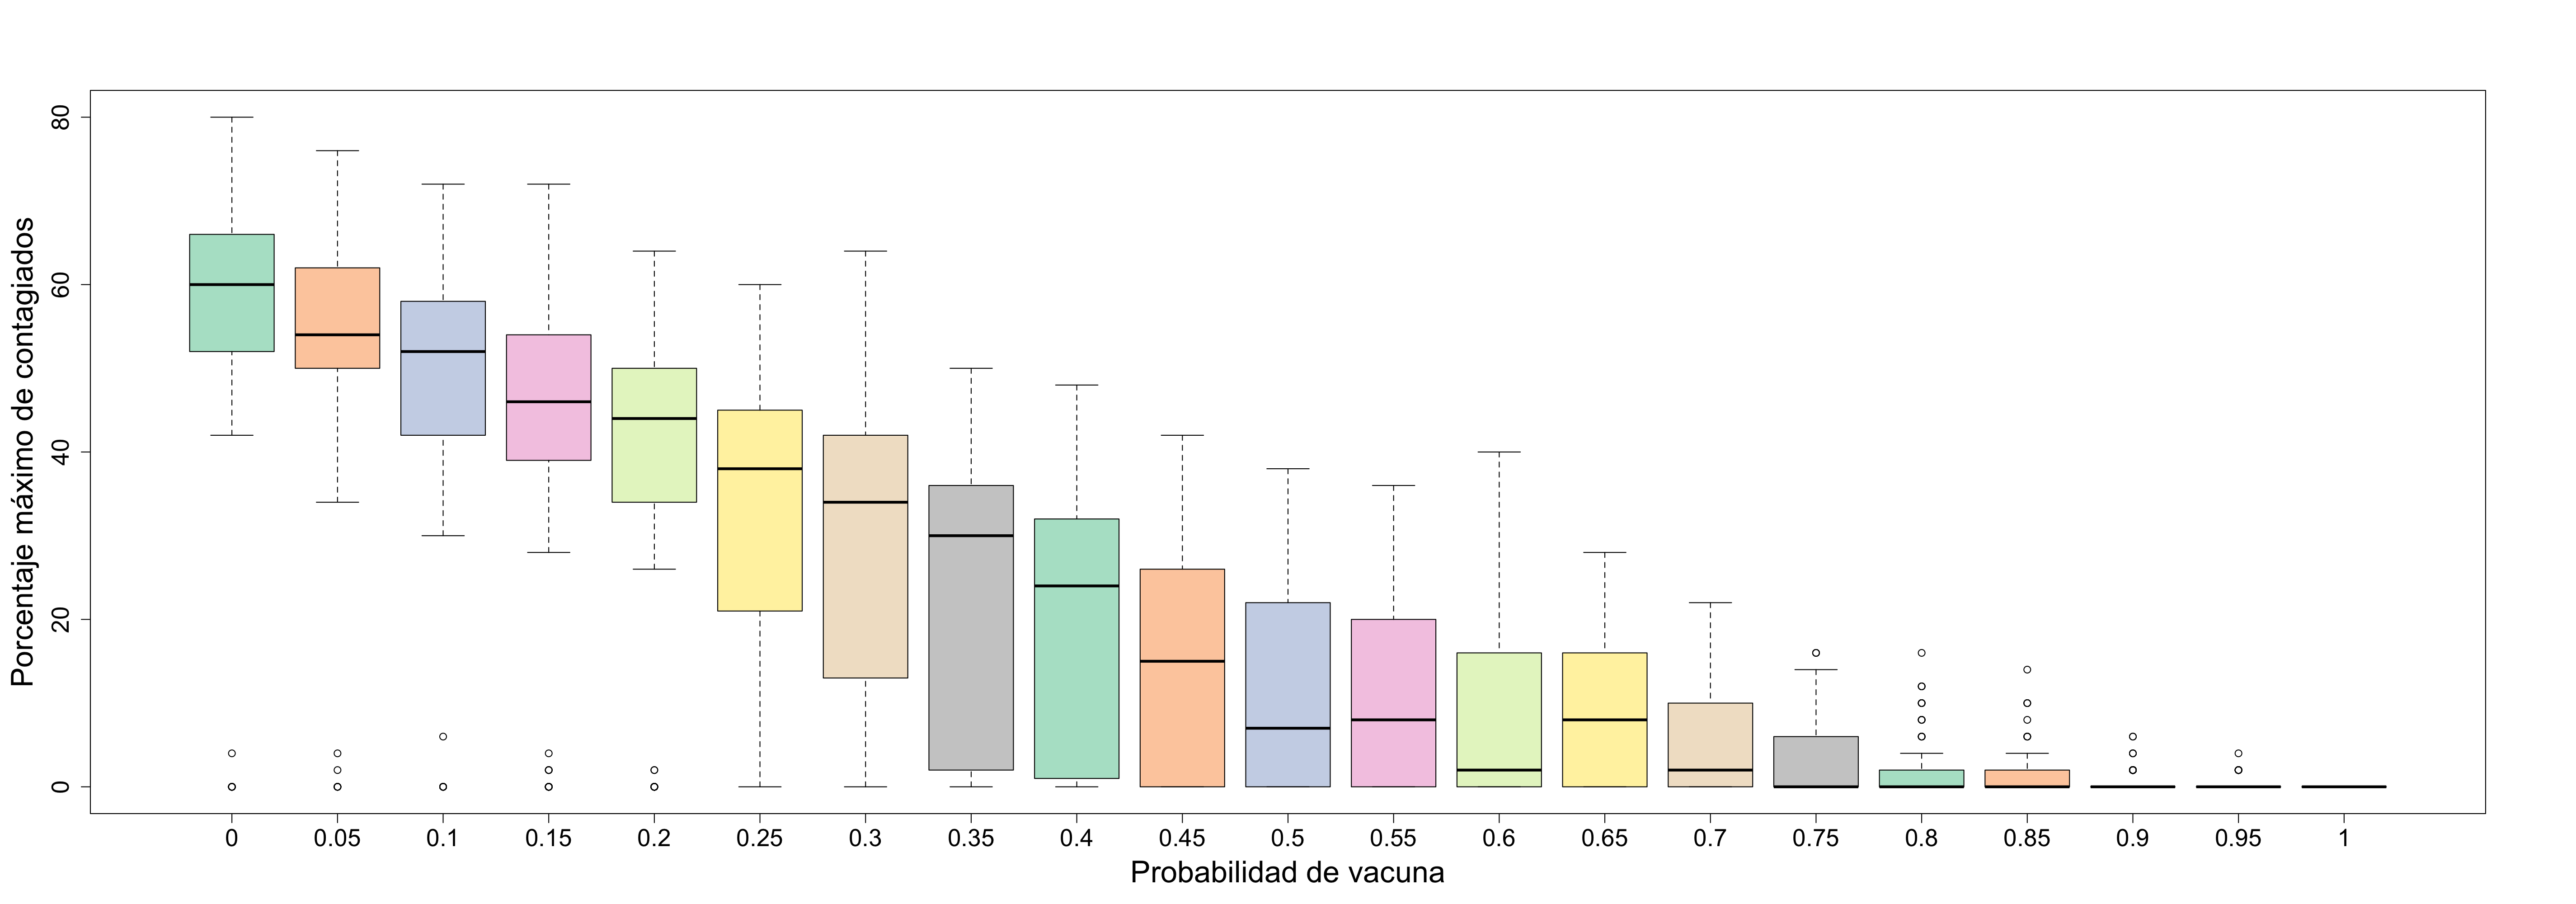
\includegraphics[width=\linewidth]{boxplot1.png}
	\caption{Gráficas de caja bigote del porcentaje máximo de infectados.}
	\label{box1}
\end{figure}

\begin{figure}
	\centering
	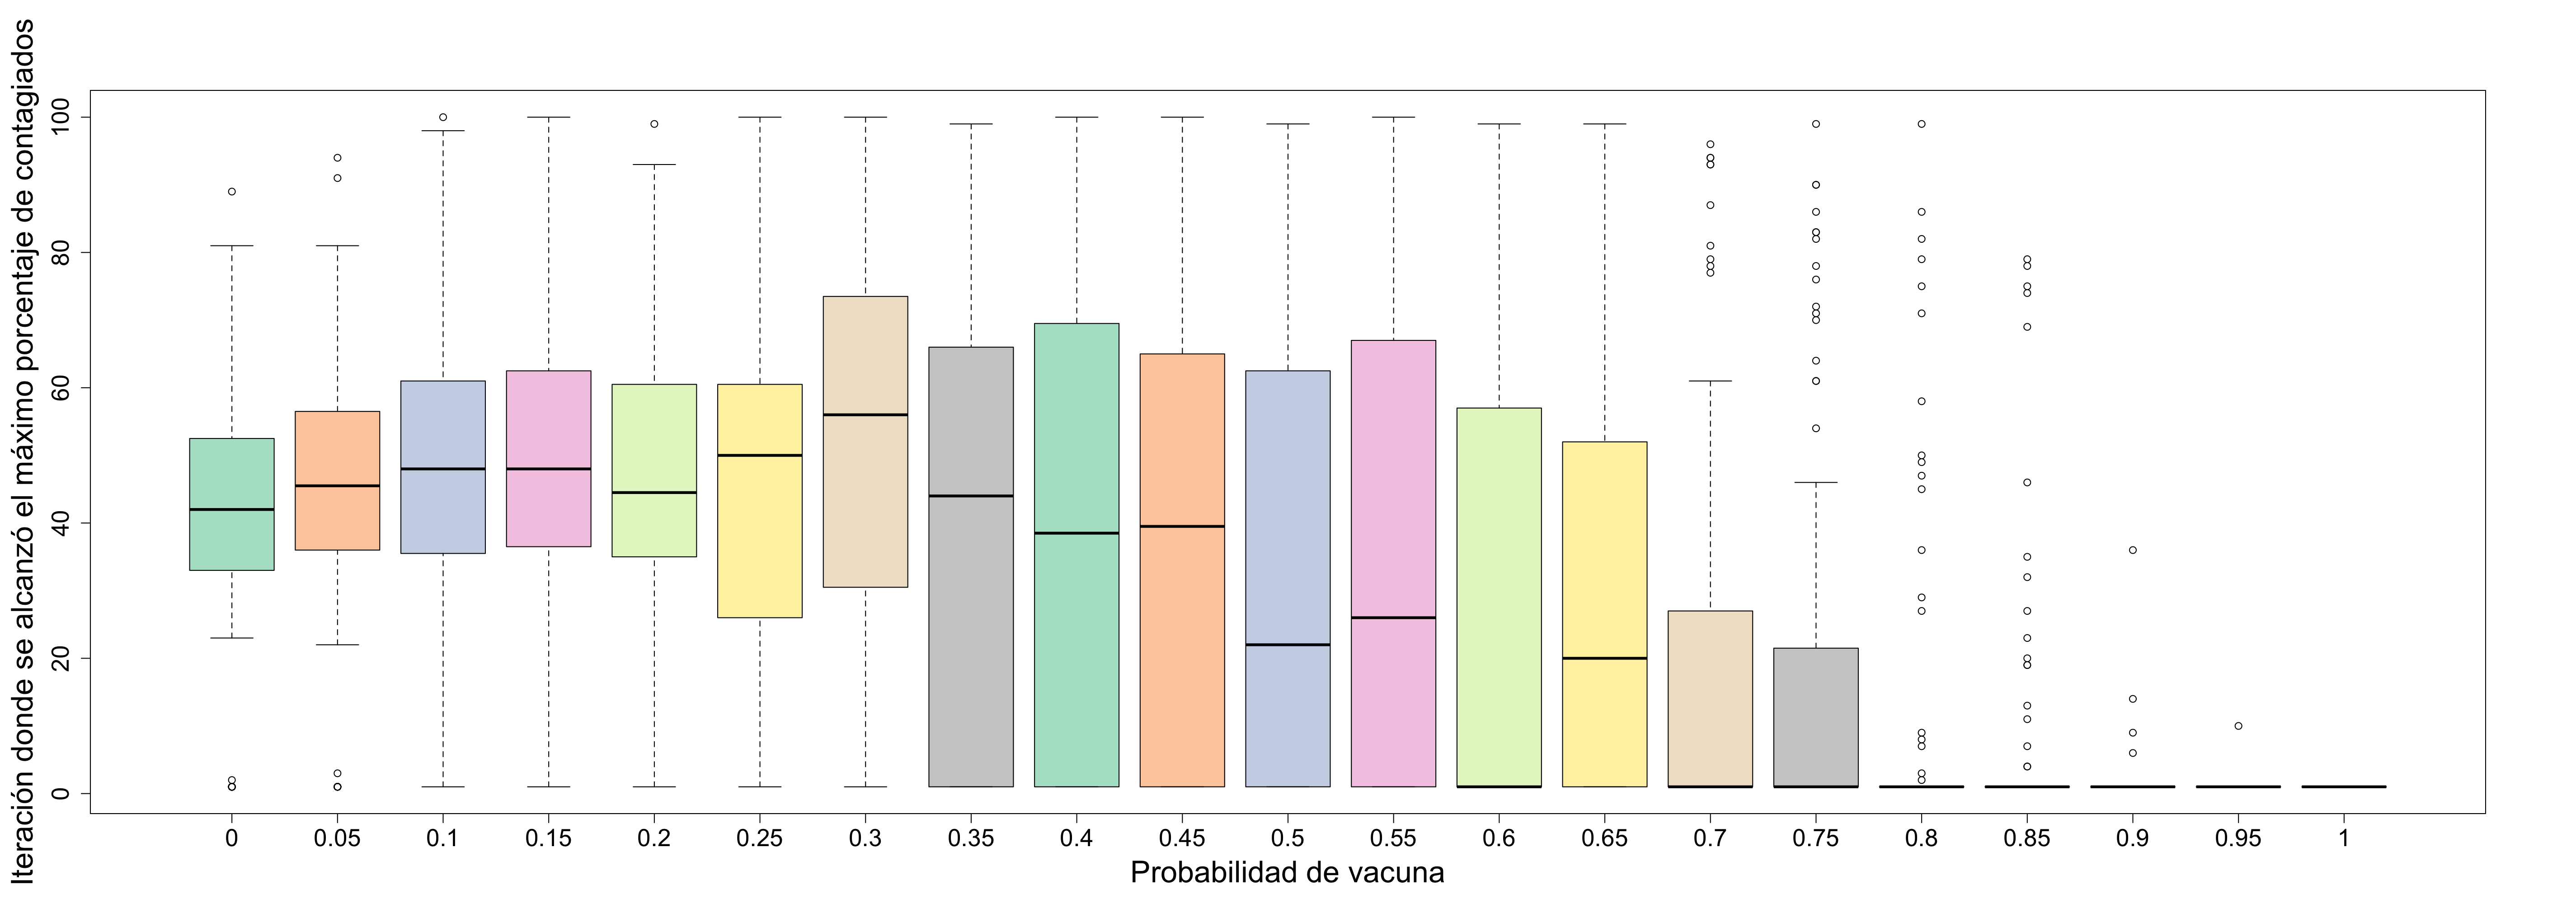
\includegraphics[width=\linewidth]{max_iter.png}
	\caption{Gráficas de caja bigote de la iteración donde se alcanzó el porcentaje máximo.}
	\label{box2}
\end{figure}

%\begin{figure}
%	\centering
%	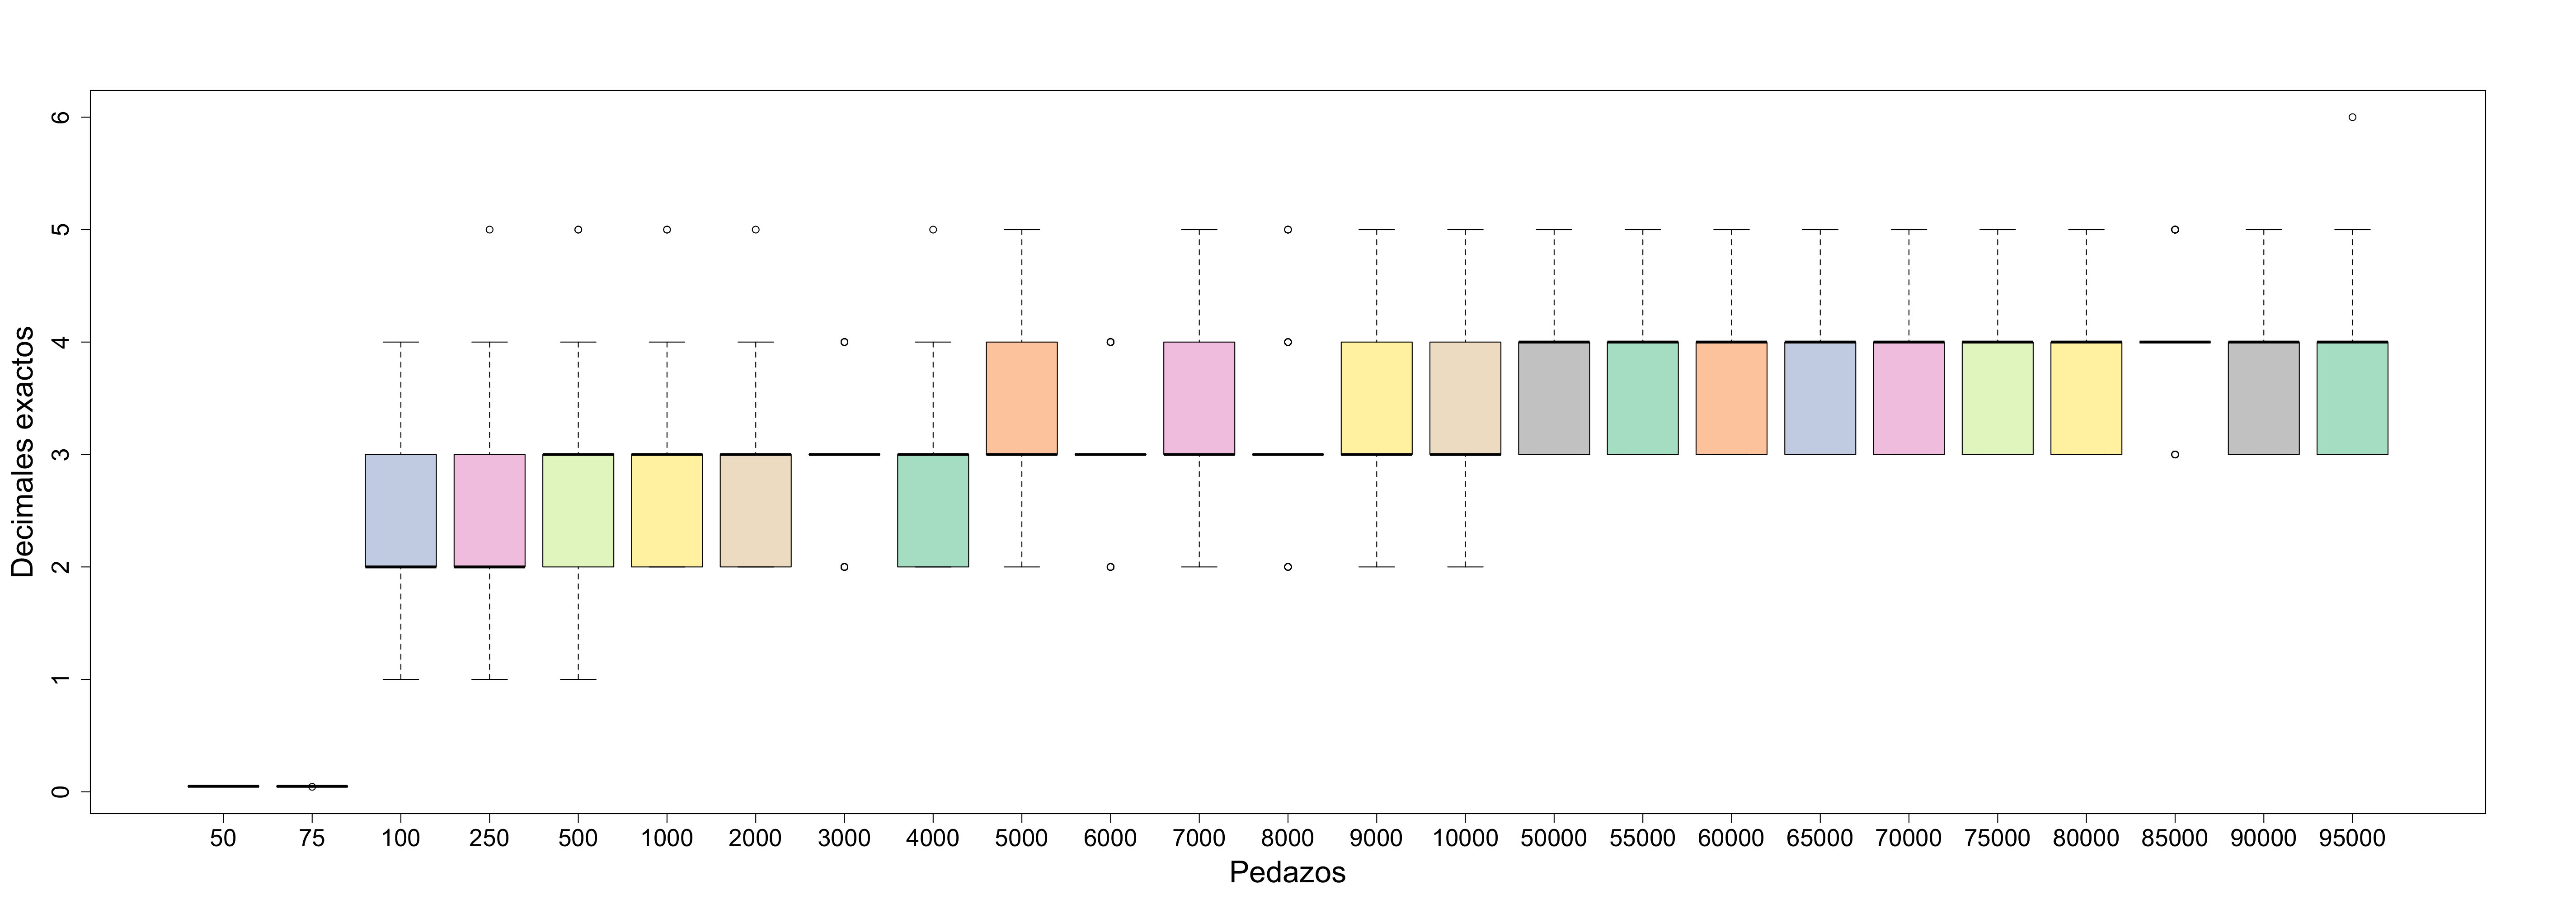
\includegraphics[width=\linewidth]{boxplot2.png}
%	\caption{Gráficas de caja bigote de la cantidad de decimales en que coinciden los valores obtenidos de la integral con el valor de \texttt{wolfram}.}
%	\label{box2}
%\end{figure}
\subsection{Pruebas de correlación}
Se realiza la prueba de correlación para las columnas del valor de \texttt{pv} y el máximo porcentaje de infectados. La prueba de correlación arroja los siguientes resultados,

\begin{verbatim}
Pearson's product-moment correlation

data:  datos$PV and datos$Porcentaje
t = -55.98, df = 2098, p-value < 2.2e-16
alternative hypothesis: true correlation is not equal to 0
95 percent confidence interval:
 -0.7905482 -0.7562048
sample estimates:
      cor 
-0.773945.
\end{verbatim}
La prueba arroja un valor $p$ de $2.2\times 10^{-16}$ el cual es menor que 0.05, por lo que se rechaza la hipótesis nula y se concluye que hay correlación entre estas variables. Es decir, el valor de \texttt{pv} afecta al porcentaje de infectados. En particular, se estima el coeficiente de correlación en $-0.7739$ por lo que se concluye cuando el valor de \texttt{pv} aumenta, el máximo porcentaje de infectados disminuye. 




\section{Reto 1}
Para el reto 1, se modifica la manera en que se mueven los agentes\footnote{Un gif de este tipo de movimiento se encuentra en \url{https://github.com/fvzqa/Simulacion/blob/master/Tarea6/Images/reto1.gif}}, fijando una meta uniformemente al azar y al llegar a ella, vuelve a fijar otra meta. El objetivo es concluir si este nuevo tipo de movimiento de los agentes afecta o no las conclusiones anteriores.

En la figura \ref{box3} se tienen las gráficas de caja obtenidos en el experimento, como se ve, tiene un comportamiento similar a las gráficas obtenida en la figura \ref{box1}. Pero, como era de esperarse, este nuevo tipo movimiento de los agentes, hace que tengan mayor contacto con los demás, por ello los porcentajes máximos de contagio con este movimiento son mayores.
\begin{figure}
	\centering
	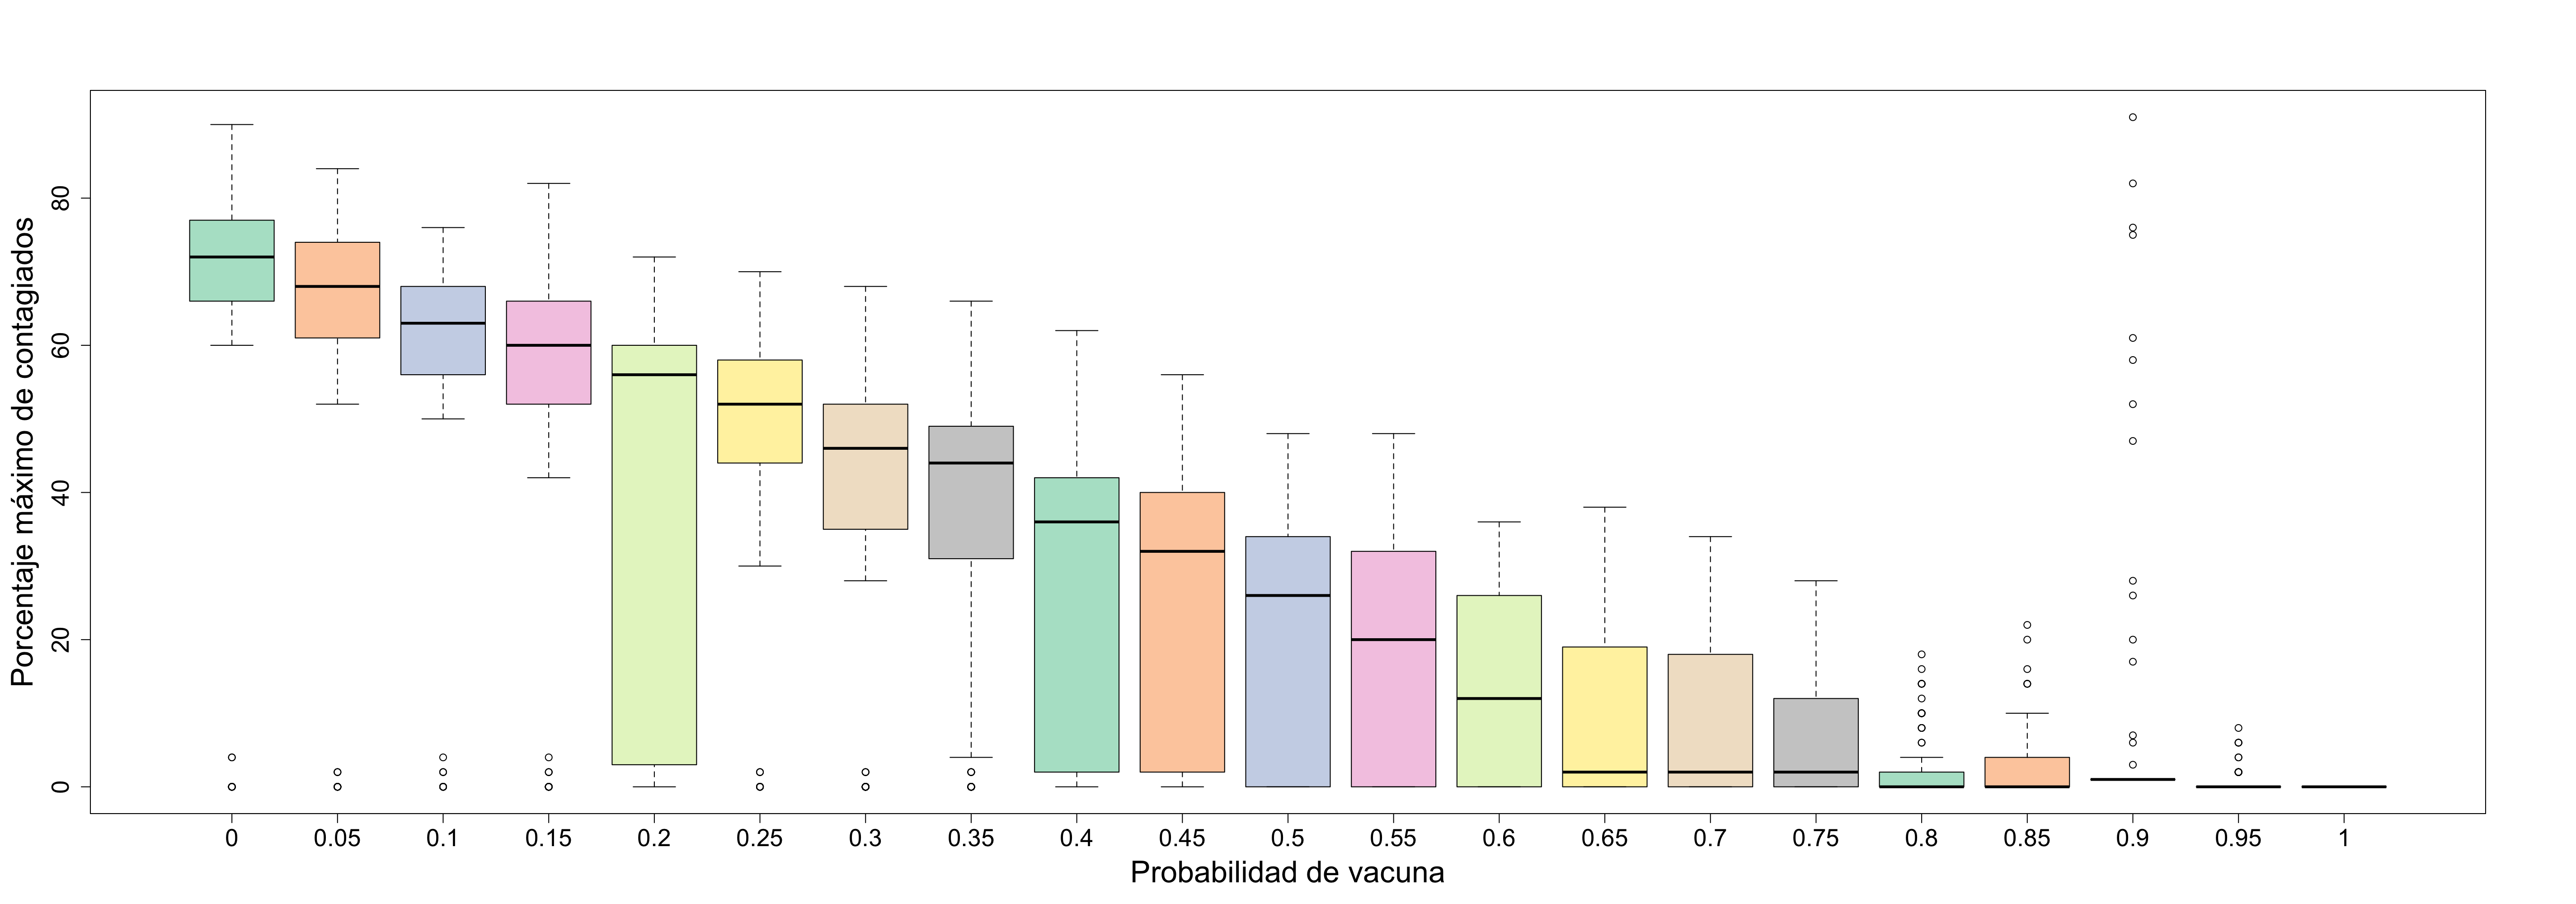
\includegraphics[width=\linewidth]{boxplot_reto1.png}
	\caption{Gráficas de caja bigote de las aproximaciones del porcentaje máximo alcanzado, variando la probabilidad \texttt{pv}.}
	\label{box3}
\end{figure}

\begin{figure}
	\centering
	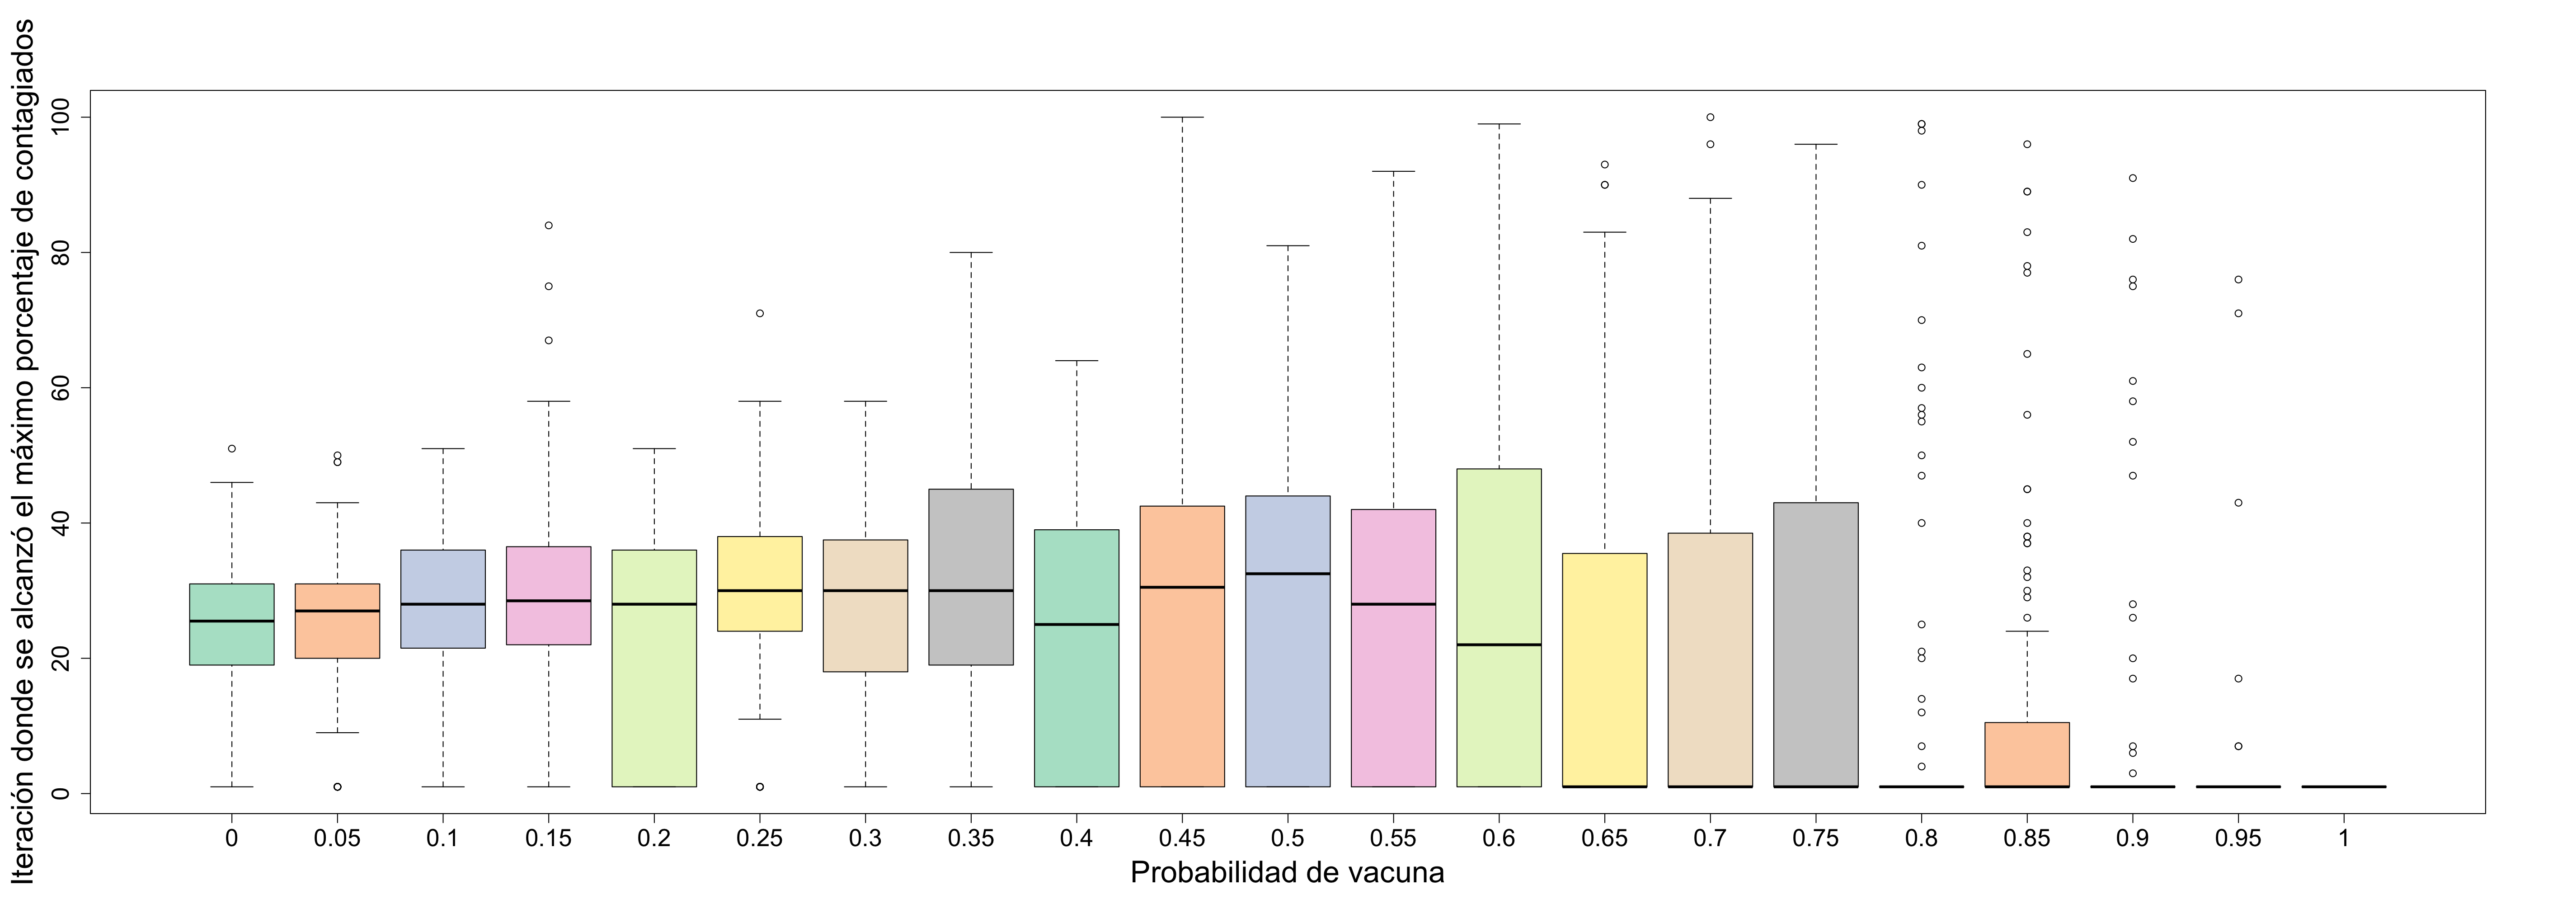
\includegraphics[width=\linewidth]{maxiter_reto1.png}
	\caption{Gráficas de caja bigote de la iteración donde se alcanza el máximo porcentaje de contagiados.}
	\label{box4}
\end{figure}

\subsection{Pruebas de correlación}
Se realiza la prueba de correlación para las columnas del valor de \texttt{pv} y el máximo porcentaje de infectados, ahora con esta forma de desplazamiento de los agentes.
\begin{verbatim}
Pearson's product-moment correlation

data:  datos_1$PV and datos_1$Porcentaje
t = -54.801, df = 2098, p-value < 2.2e-16
alternative hypothesis: true correlation is not equal to 0
95 percent confidence interval:
 -0.7843157 -0.7490935
sample estimates:
       cor 
-0.7672826
\end{verbatim}
La prueba arroja un valor $p$ de $2.2\times 10^{-16}$ el cual es menor que 0.05, por lo que se rechaza la hipótesis nula y se concluye que hay correlación entre estas variables. Es decir, el valor de \texttt{pv} afecta al porcentaje de infectados. En particular, se estima el coeficiente de correlación en $-0.7672$ por lo que se concluye cuando el valor de \texttt{pv} aumenta, el máximo porcentaje de infectados disminuye. 
\bibliographystyle{plain} 
\bibliography{Referencias}


\end{document} 